\documentclass[a4paper,14pt]{extarticle} 
\usepackage[a4paper,top=1.5cm, bottom=1.5cm, left=2cm, right=1cm]{geometry}
%\usepackage[T2A]{fontenc}
%\usepackage[english, russian]{babel}
\usepackage{graphicx}
\DeclareGraphicsExtensions{.pdf,.png,.jpg}

\usepackage{fontspec}
\setmainfont{Times New Roman}
\setsansfont{FreeSans}
\setmonofont{FreeMono}
\renewcommand{\baselinestretch}{1.5}
\usepackage{polyglossia}
\setdefaultlanguage{russian}
\setotherlanguages{english,russian}
\usepackage{setspace}
\usepackage[many]{tcolorbox}
\usepackage{listings}
\usepackage{xcolor}

\definecolor{codegreen}{rgb}{0,0.6,0}
\definecolor{codegray}{rgb}{0.5,0.5,0.5}
\definecolor{codepurple}{rgb}{0.58,0,0.82}
\definecolor{backcolour}{rgb}{0.95,0.95,0.92}

\lstdefinestyle{mystyle}{
    backgroundcolor=\color{backcolour},   
    keywordstyle=\color{magenta},
    numberstyle=\tiny\color{codegray},
    stringstyle=\color{codepurple},
    basicstyle=\ttfamily\footnotesize,
    breakatwhitespace=false,         
    breaklines=true,                 
    captionpos=b,                    
    keepspaces=true,                 
    numbers=left,                    
    numbersep=5pt,                  
    showspaces=false,                
    showstringspaces=false,
    showtabs=false,                  
    tabsize=2
}

\lstset{style=mystyle}
\setlength{\parindent}{5ex}


\begin{document}
    \begin{center}
        \thispagestyle{empty}
        \begin{singlespace}
        ФЕДЕРАЛЬНОЕ АГЕНТСТВО СВЯЗИ

        ФЕДЕРАЛЬНОЕ ГОСУДАРСТВЕННОЕ БЮДЖЕТНОЕ ОБРАЗОВАТЕЛЬНОЕ

        УЧРЕЖДЕНИЕ ВЫСШЕГО ОБРАЗОВАНИЯ

        «САНКТ-ПЕТЕРБУРГСКИЙ ГОСУДАРСТВЕННЫЙ УНИВЕРСИТЕТ ТЕЛЕКОММУНИКАЦИЙ ИМ. ПРОФ. М.А. БОНЧ-БРУЕВИЧА»

        (СПбГУТ)
        \end{singlespace}
        \vspace{-1ex}
        \rule{\textwidth}{0.4pt}
        \vspace{-5ex}

        Факультет \underline{Инфокоммуникационных сетей и систем}

        Кафедра \underline{Защищенных систем связи}
        \vspace{10ex}

        \textbf{Лабораторная работа №1}\\
        


    \end{center}
    \vspace{4ex}
    \begin{flushright}
    \parbox{10 cm}{
    \begin{flushleft}
        Выполнили студенты группы ИКТЗ-83:

        \underline{Громов А.А., Миколаени М.С., Мазеин Д.С.} \hfill \rule[-0.85ex]{0.1\textwidth}{0.6pt}

        \footnotesize \textit{ (Ф.И.О., № группы) \hfill (подпись)} \normalsize

        Проверил:

        \underline{Казанцев А.А.} \hfill \rule[-0.85ex]{0.1\textwidth}{0.6pt}

        (\footnotesize \textit{уч. степень, уч. звание, Ф.И.О.) \hfill (подпись)} \normalsize

    \end{flushleft}
    }
    \end{flushright}
    \begin{center}
        \vfill
        Санкт-Петербург

        2021

    \end{center}
    \newpage

    \textbf{Цель лабораторной работы:}
    Научиться устанавливать компоненты программного комплекса на локальный компьютер, 
    устанавливать агента на компьютер рабочей группы, настраивать перехват данных при 
    помощи агента, настраивать работу ключевых сервисов Falcongaze SecureTower.

    \textbf{Пункт 1} \\
    \begin{center}
        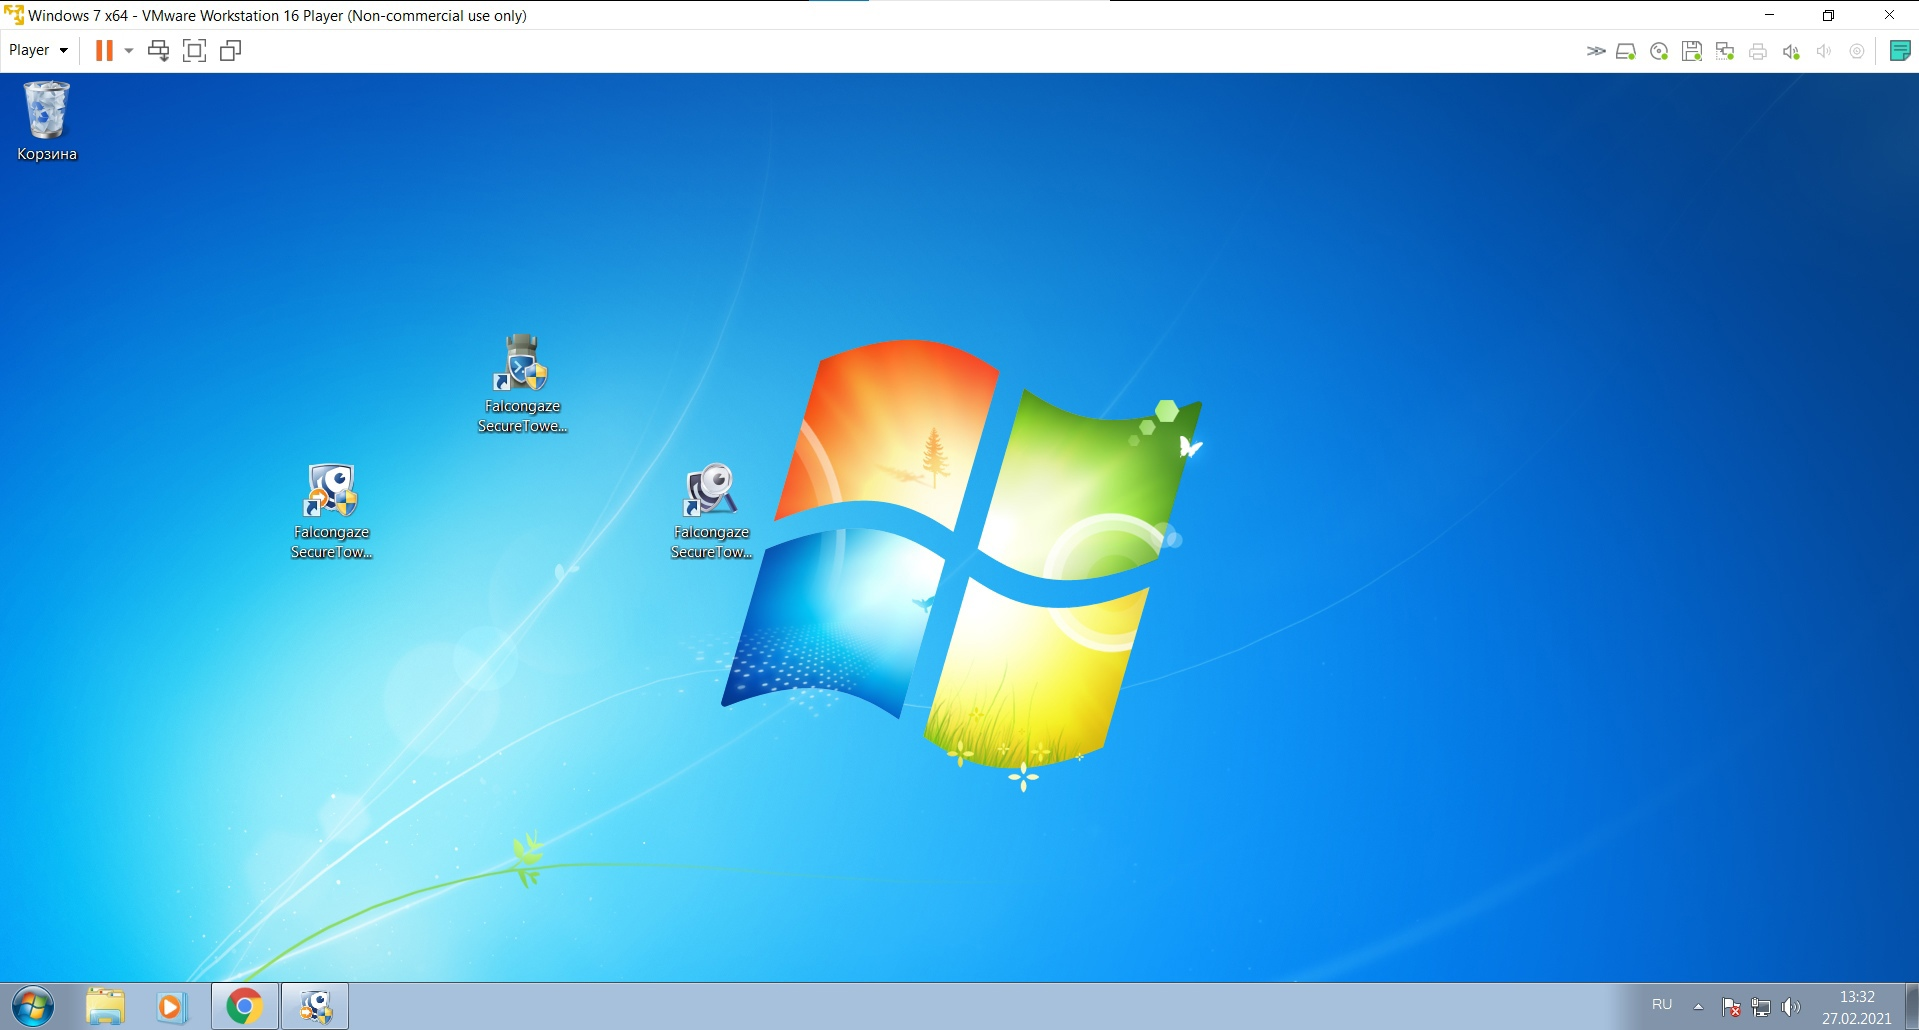
\includegraphics[scale=0.25]{pics/1.jpg}
    \end{center}

    \textbf{Пункт 2} \\
    \begin{center}
        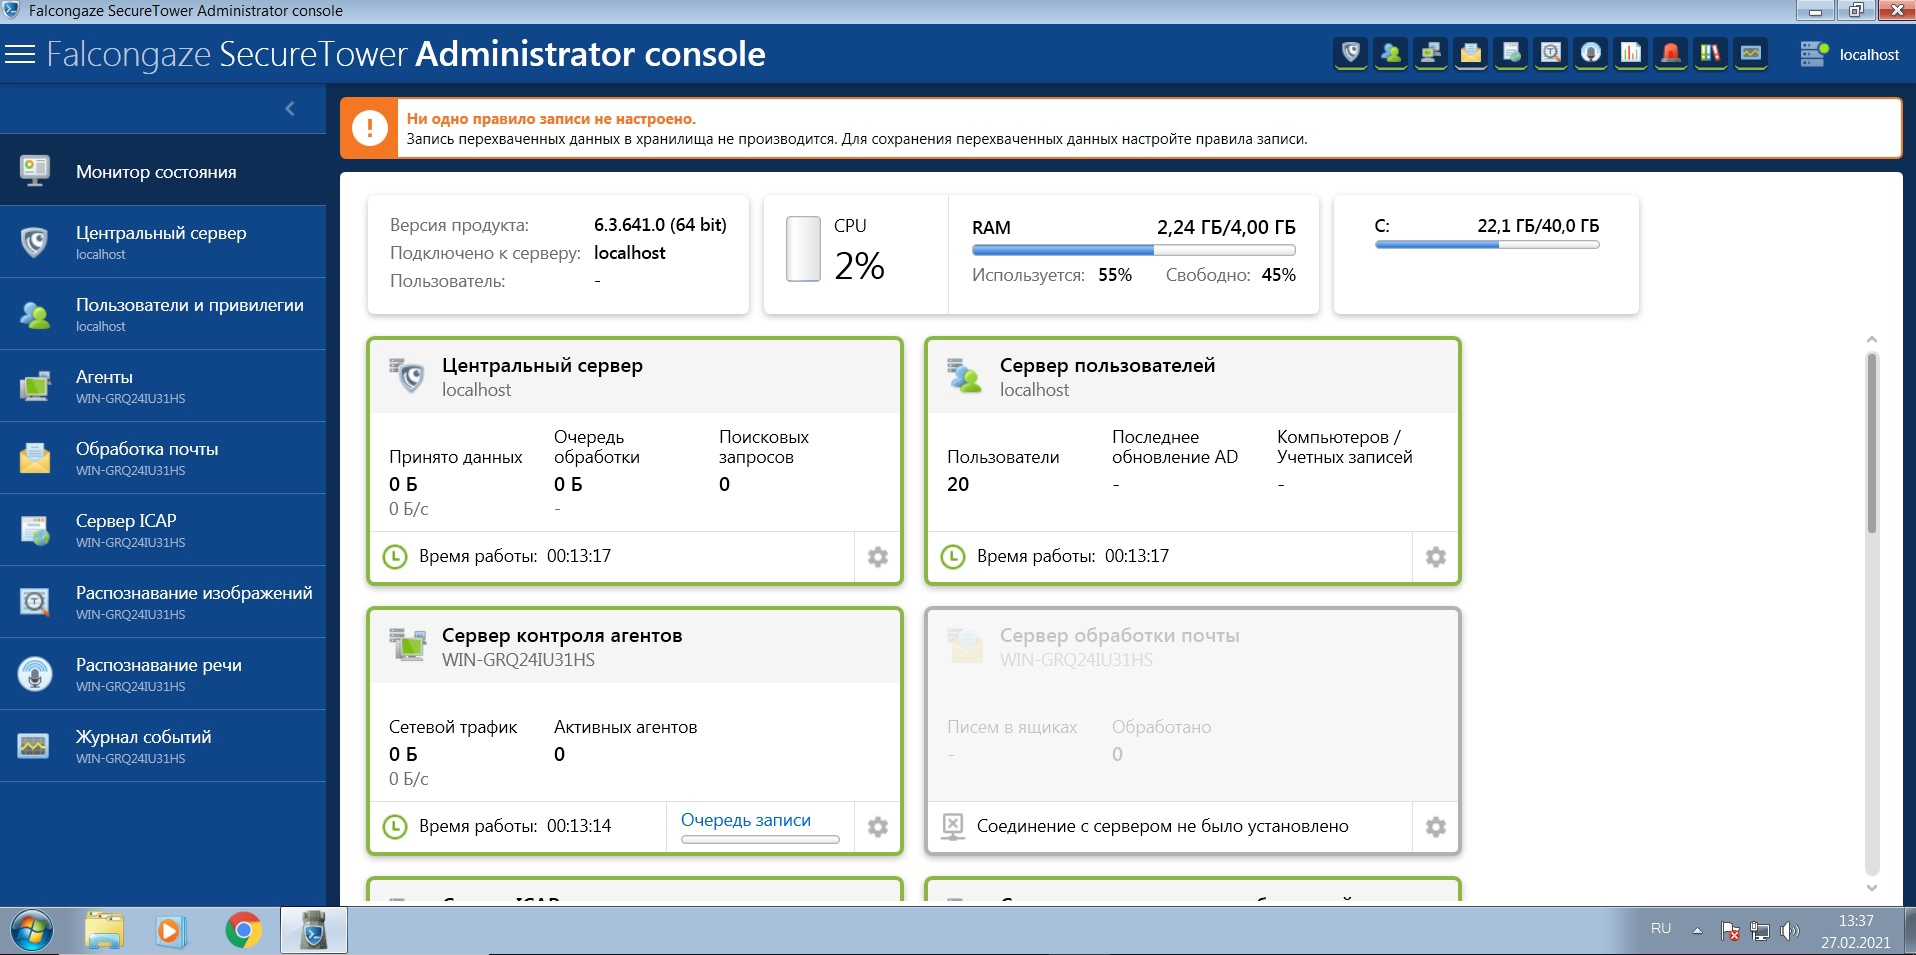
\includegraphics[scale=0.25]{pics/2.jpg}
    \end{center}

    \textbf{Пункт 3} \\
    \begin{center}
        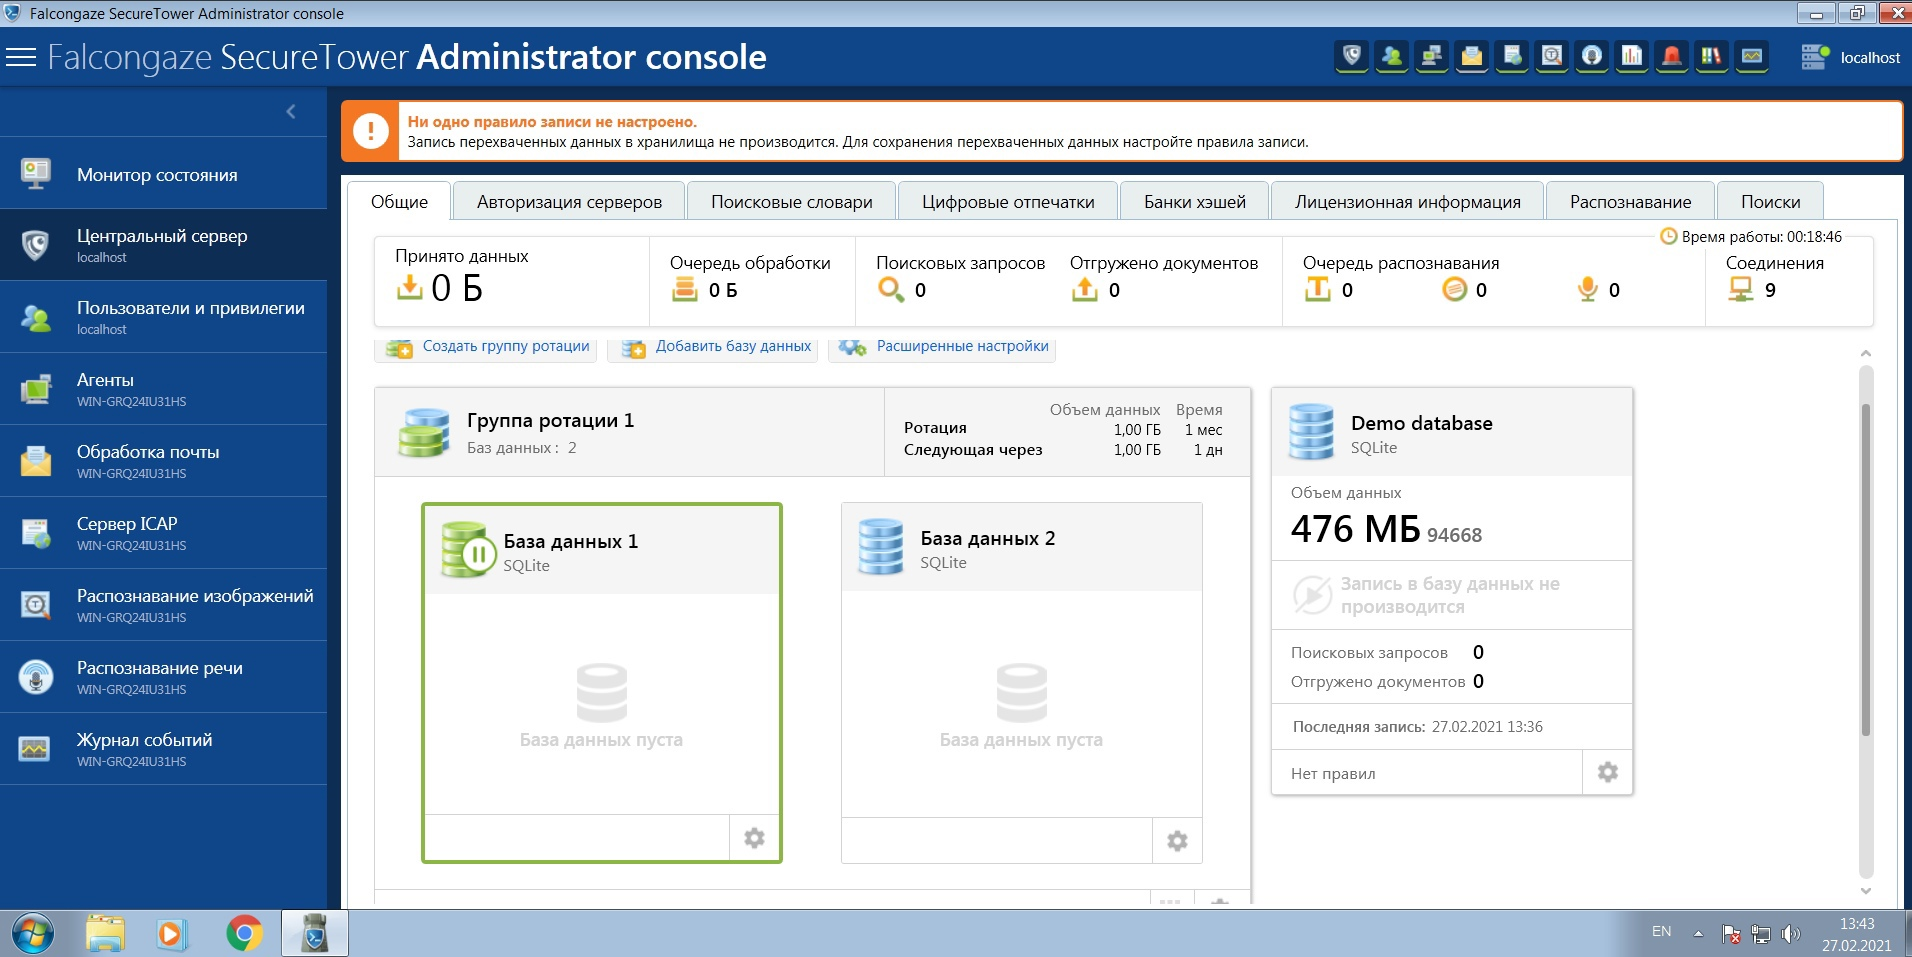
\includegraphics[scale=0.25]{pics/3.jpg}
    \end{center}

    \textbf{Пункт 3.1} \\
    \begin{center}
        
\includegraphics[scale=0.3]{pics/3_1.jpg}
    \end{center}

    \textbf{Пункт 5} \\
    \begin{center}
        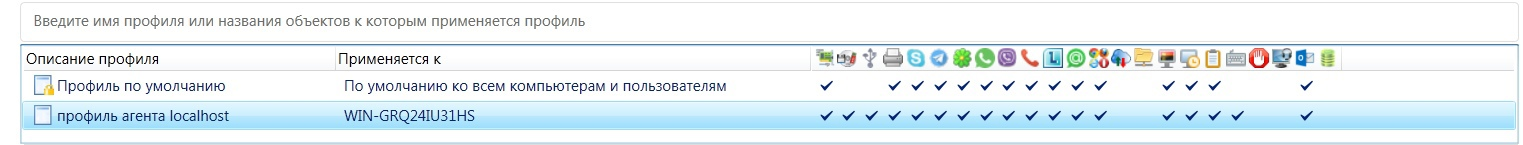
\includegraphics[scale=0.3]{pics/5.jpg}
    \end{center}

    \newpage
    \textbf{Пункт 6} \\
    \begin{center}
        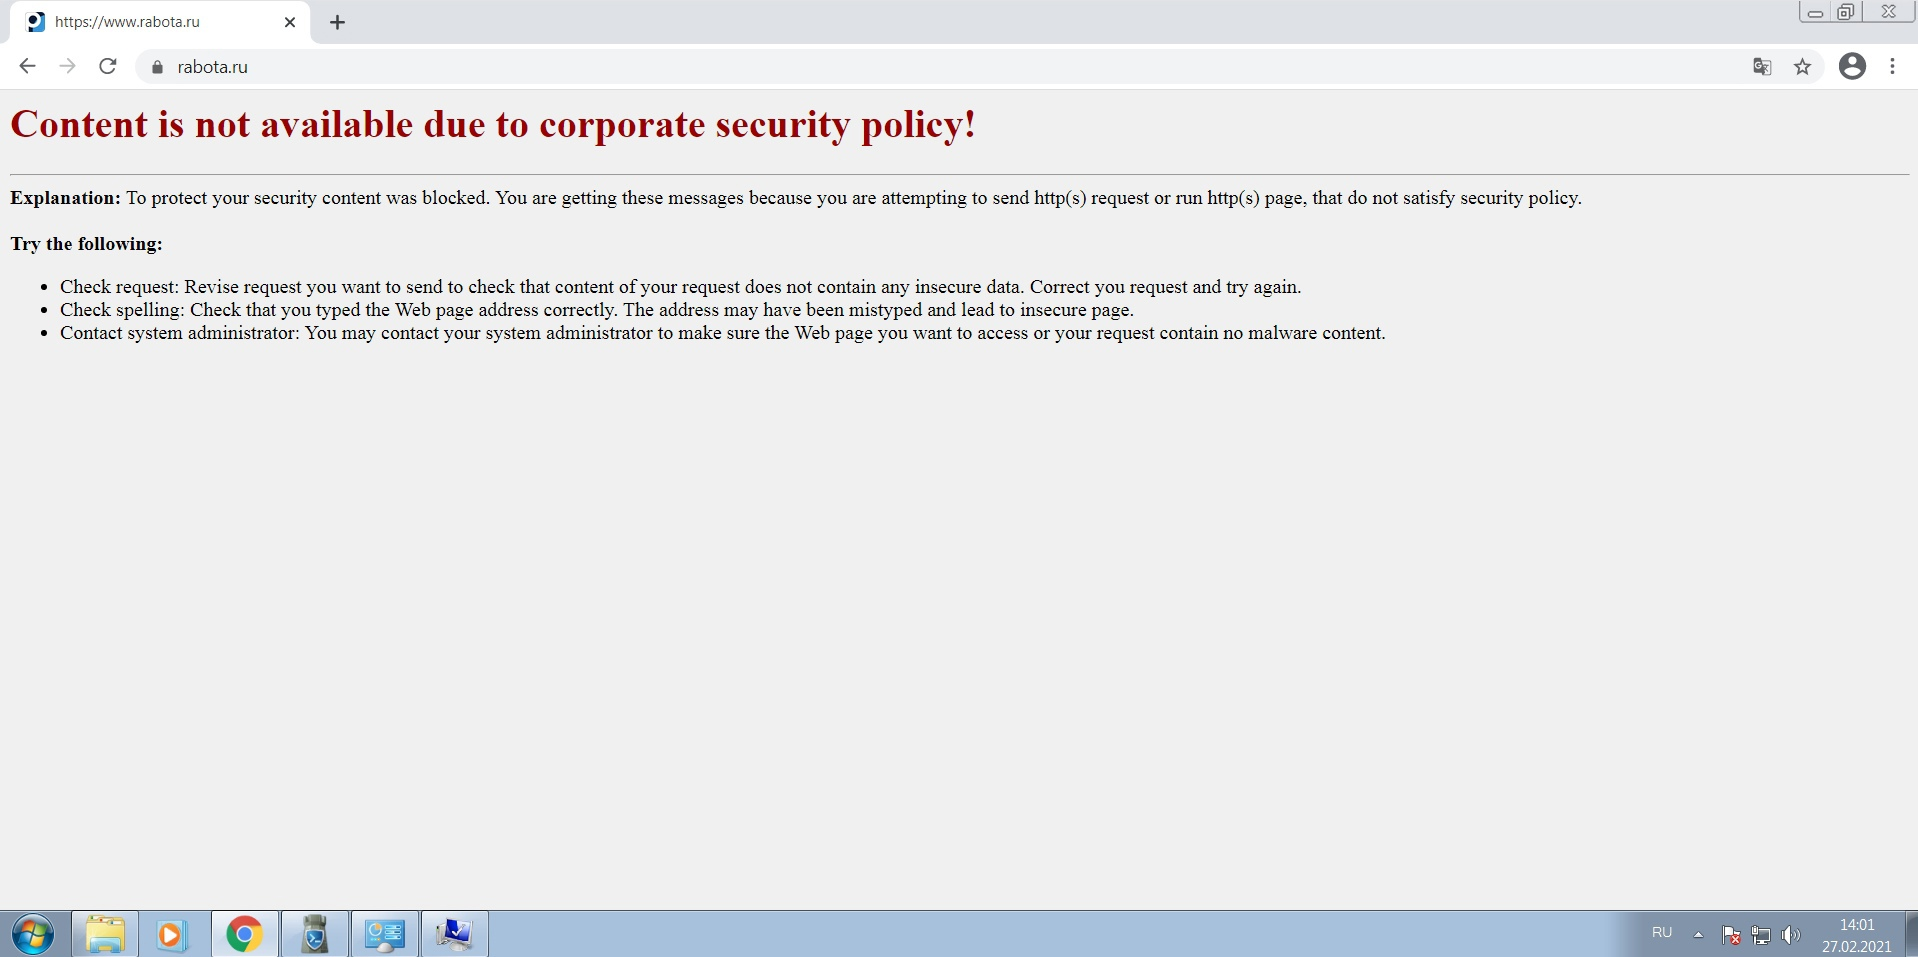
\includegraphics[scale=0.25]{pics/6.jpg}
    \end{center}

    \textbf{Пункт 7} \\
    \begin{center}
        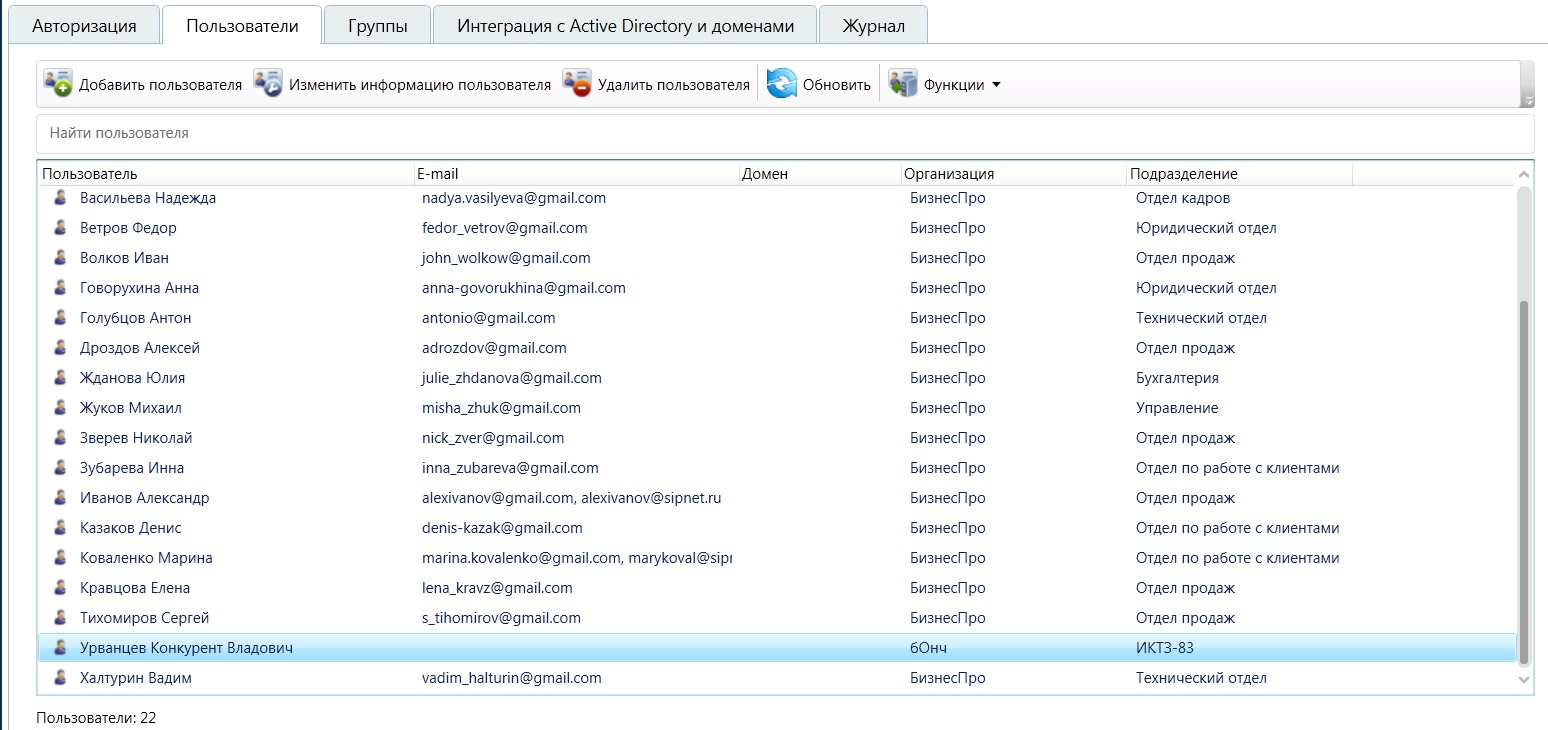
\includegraphics[scale=0.25]{pics/7.jpg}
    \end{center}

    \newpage
    \textbf{Пункт 8} \\
    \begin{center}
        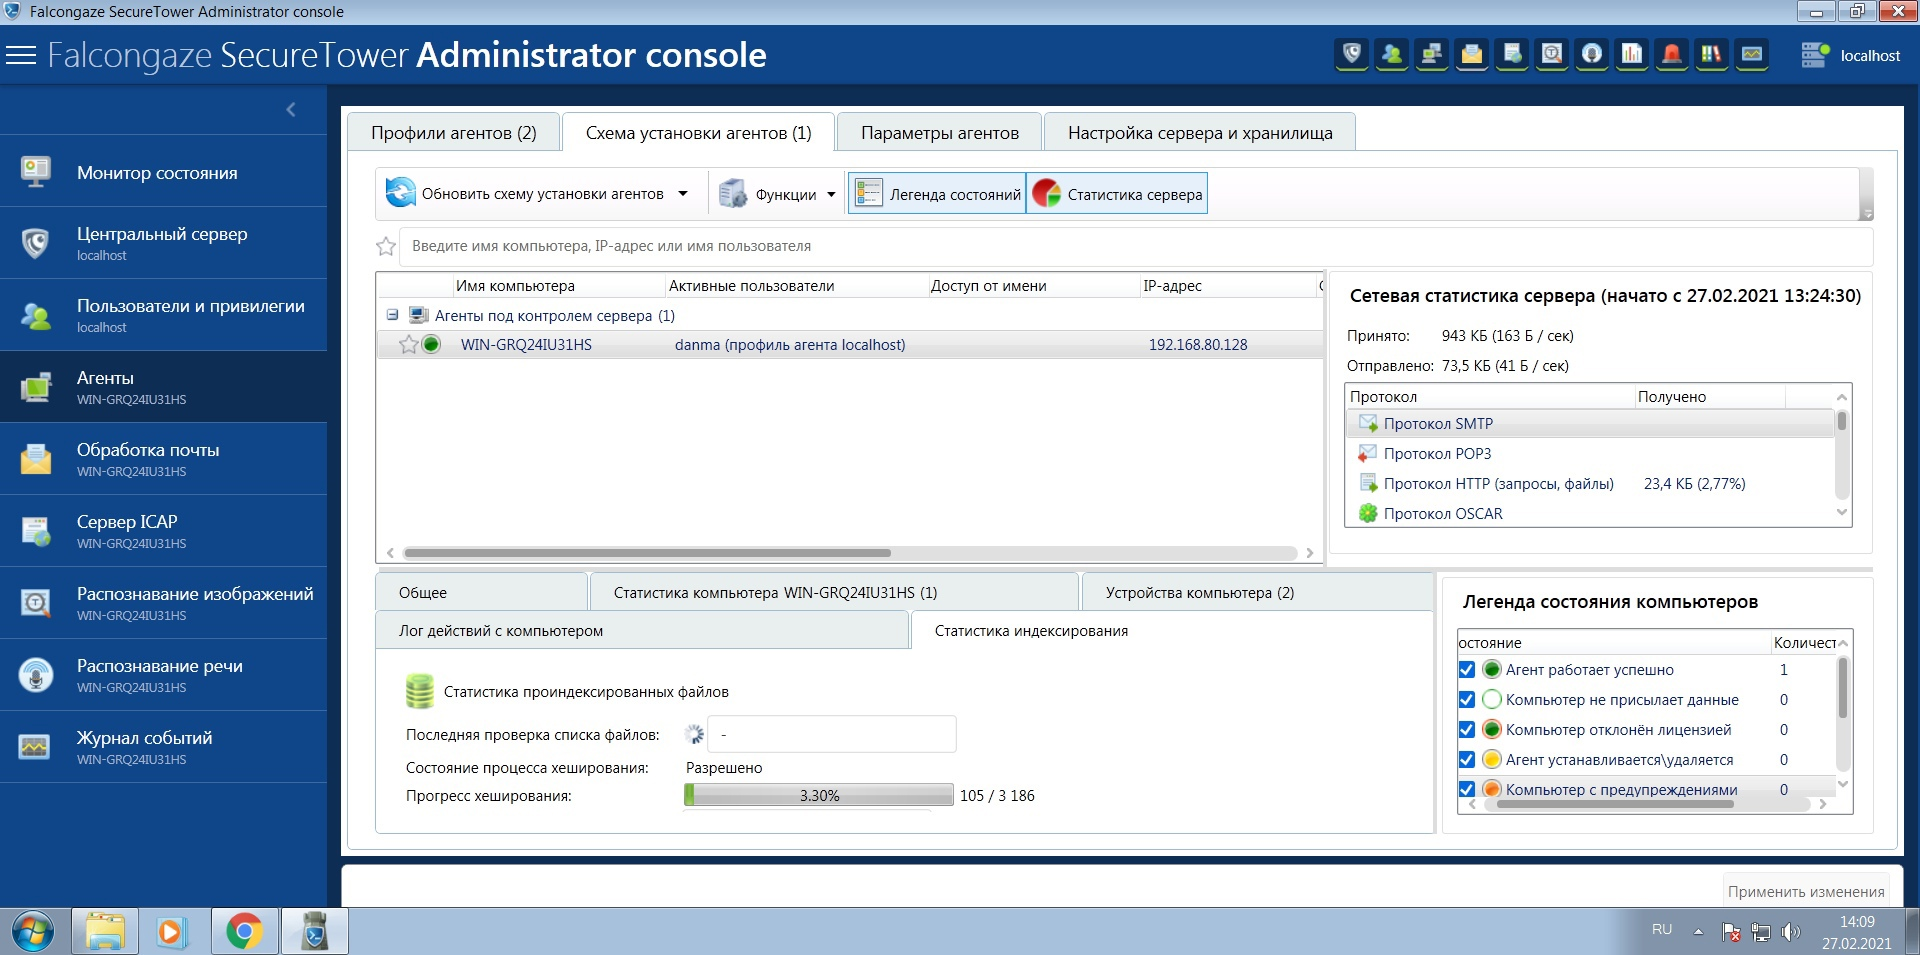
\includegraphics[scale=0.25]{pics/8.jpg}
    \end{center}

    \textbf{Пункт 8.1} \\
    \begin{center}
        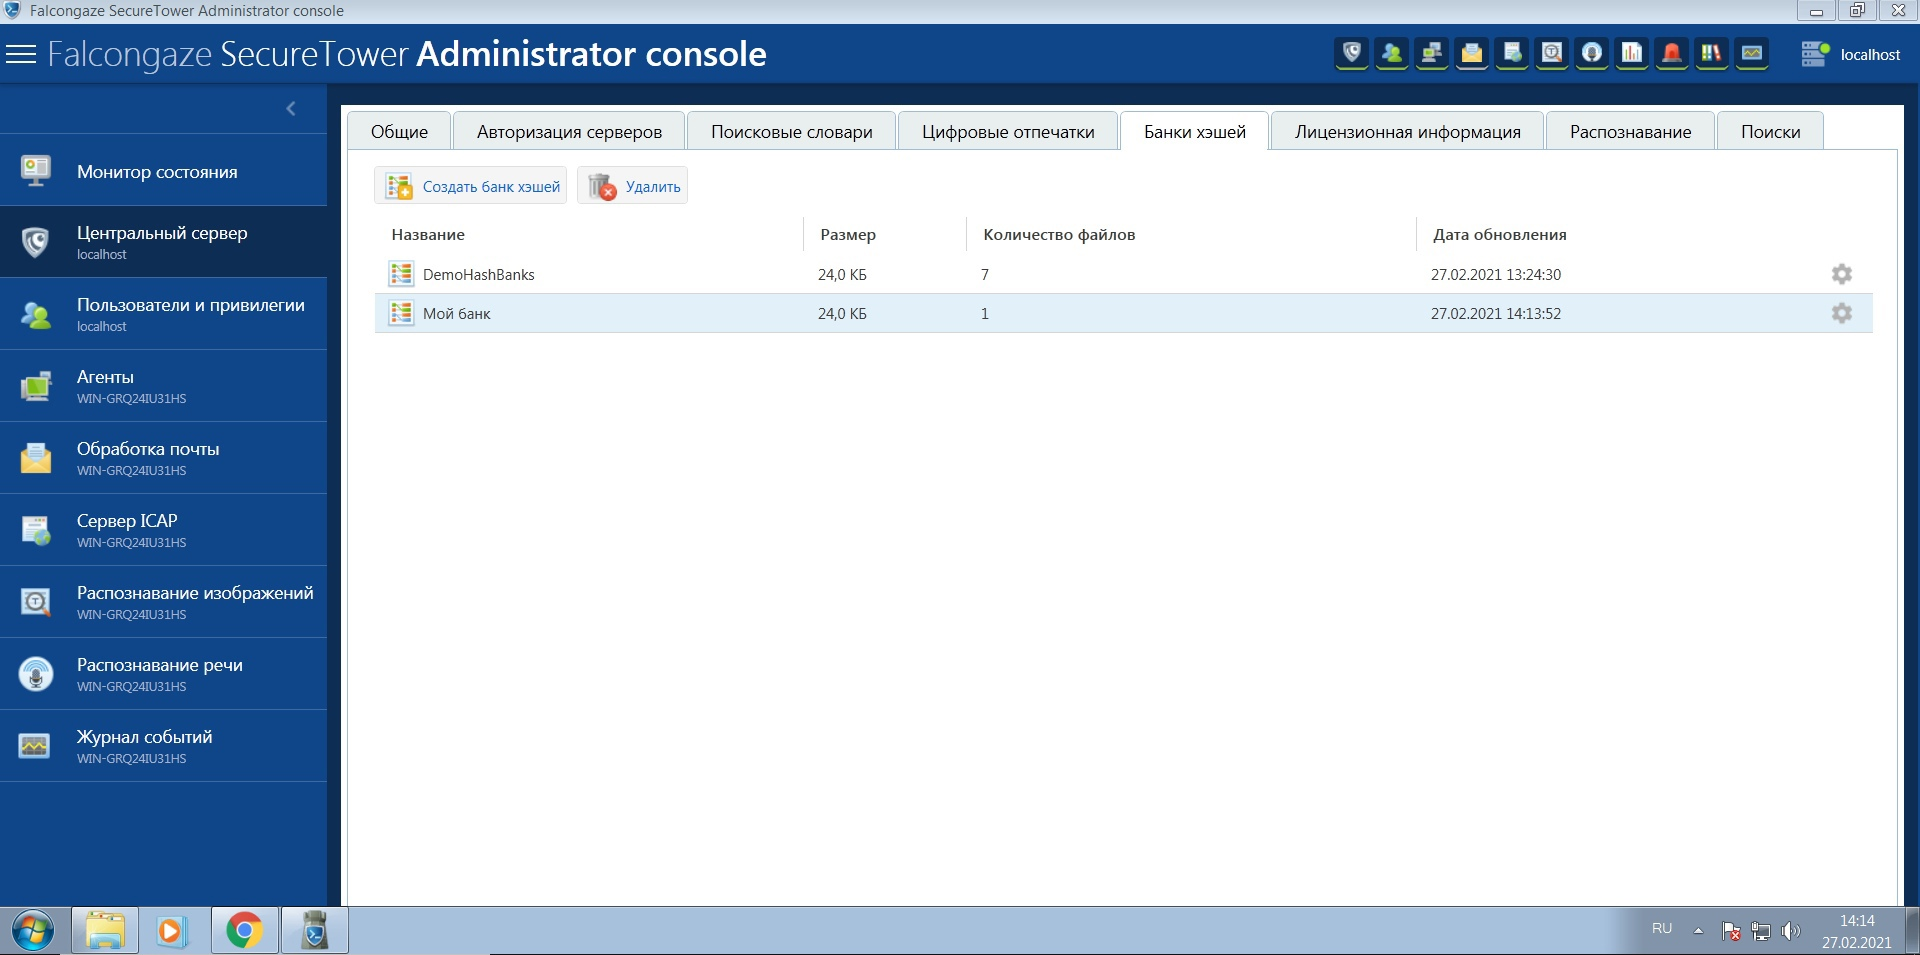
\includegraphics[scale=0.25]{pics/8_1.jpg}
    \end{center}

    \newpage
    \textbf{Пункт 8.2} \\
    \begin{center}
        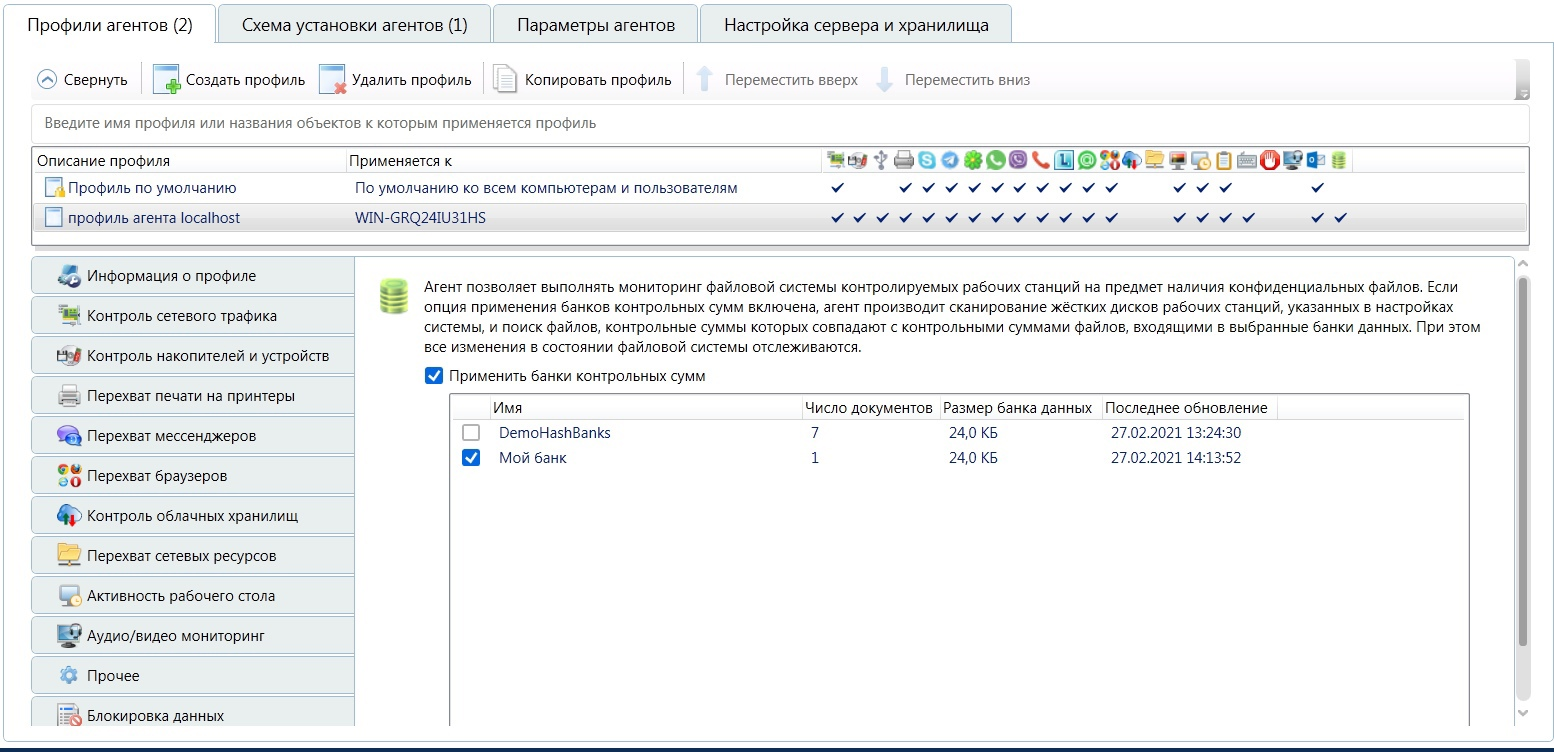
\includegraphics[scale=0.25]{pics/8_2.jpg}
    \end{center}

    \textbf{Пункт 9} \\
    \begin{center}
        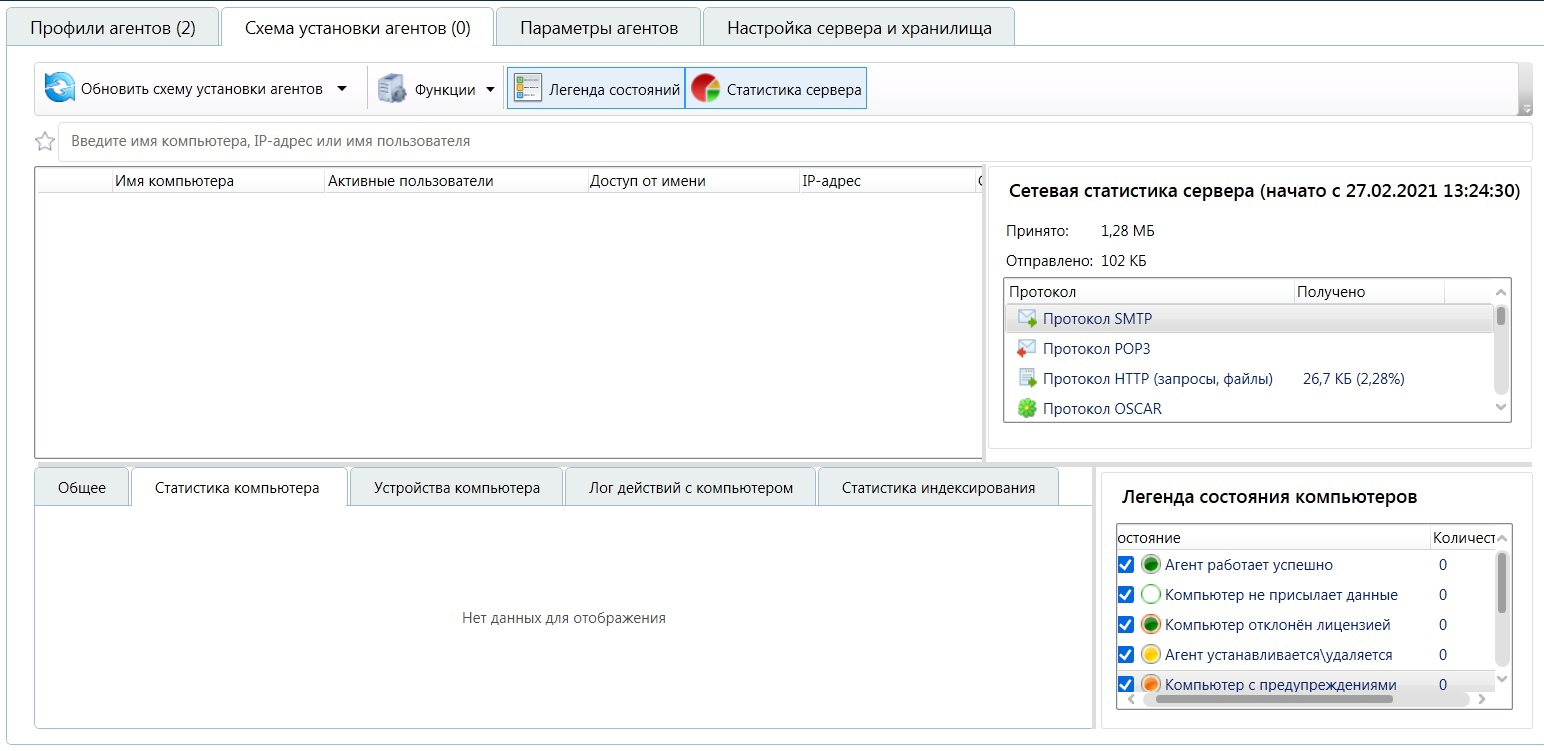
\includegraphics[scale=0.25]{pics/9.jpg}
    \end{center}

    \textbf{Ответы на контрольные вопросы}
    \begin{enumerate}
        \item \textbf{Для чего используется Консоль администратора?} \par
        \qquad Консоль администратора используется для настройки и управления
        компонентами Falcongaze.  
        \item \textbf{В каких случаях при подключении к серверу указывается локальный компьютер?} \par
        \qquad Локальный компьютер указывается в том случае, когда консоль запускается на том же 
        компьютере, где установлены серверные компоненты системы
        \item \textbf{Какие способы перехвата поддерживает система и в чем их отличие?}\par
        \qquad Система Falcongaze SecureTower может перехватывать трафик данных двумя способами: централизованно, либо агентами, устанавливаемыми на рабочие станции.\par
        \qquad Централизованный перехват имеет ряд недостатков – более трудоёмкий процесс настройки, перехватывать возможно только трафик, передаваемый по нешифрованным протоколам. \par
        \qquad Агенты, установленные на рабочих станциях, позволяют перехватывать весь трафик – как нешифрованный, так и шифрованный (по протоколам, использующим SSL-шифрование: HTTPS, FTPS, SMTPS, POP3S, IMAP4S, SIP, протоколы мессенджеров Skype, Telegram, Viber, WhatsApp, ICQ10, Google Hangouts и Microsoft Lync). Также агенты перехватывают данные, передаваемые, на внешние устройства (USB накопители, съемные жесткие диски, карты памяти и т.д.), в облачные хранилища и локальные сетевые ресурсы, локальные и сетевые принтеры, содержимое буфера обмена, реализуют функцию кейлогера, осуществляют аудит подключения внешних устройств, аудит файловых систем компьютеров и многое другое. Важной функциональной особенностью агента является возможность блокирования данных, отправленных на внешние накопители, облачные хранилища и локальные сетевые ресурсы по набору параметров и расширениям файлов, а также данных, переданных по протоколам SMTP(S), HTTP(S) и MAPI.
        \item \textbf{Для чего необходимо добавить правило записи при создании новой группы ротации/добавлении хранилища.} \par
        \qquad Для записи данных перехвата в новую группу, репликации данных, а также задания условий записи.
        \item \textbf{Какие способы установки агентов поддерживает система?}\par
        \qquad Для использования возможности перехвата через агентов необходимо, чтобы они были 
        установлены на все контролируемые рабочие станции. Существует три способа установки 
        агентов: 
        \begin{itemize}
            \item централизованно на выборочные компьютеры либо на все доступные компьютеры в сети (с Сервера контроля агентов SecureTower через Консоль администратора);
            \item через групповые политики домена;
            \item вручную с помощью отдельного инсталлятора, запущенного на рабочей станции, подлежащей контролю. 
        \end{itemize}
        \item \textbf{Возможно ли, используя настройки агента, запретить доступ к USB/ к сетевым ресурсам/ к принтерам?}\par
        \qquad Возможно заблокировать доступ ко всему перечисленному оборудованию с помощью настроек агента.
        \item \textbf{Как, используя параметры профиля настроек, защитить агента от удаления?}\par
        \qquad Во вкладке "Агенты" >> "Параметры агентов" нужно установить флажок напротив пункта "Включить защиту агентов от удаления". 
        \begin{center}
            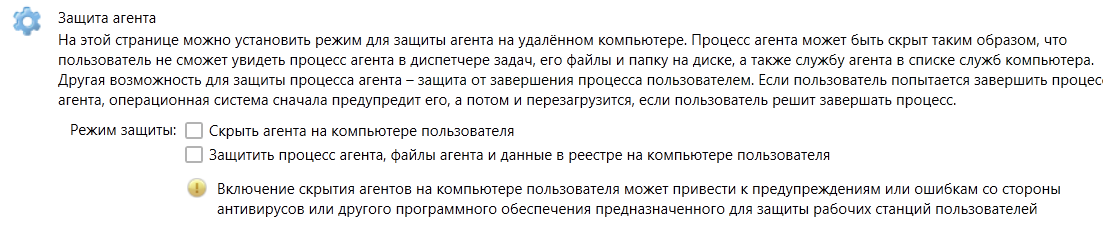
\includegraphics[scale=0.4]{pics/defence.png}
        \end{center}
        \item \textbf{Какой раздел Консоли администратора содержит информацию о работе агентов, установленных на компьютеры в сети организации?}\par
        \qquad Раздел "Агенты" >> "Схема установки агентов"
        \begin{center}
            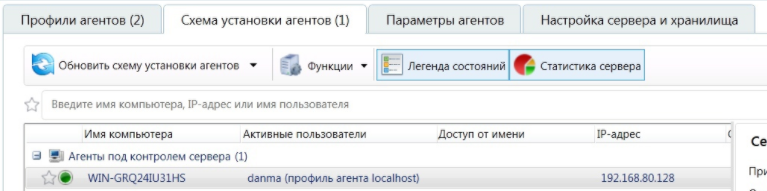
\includegraphics[scale=0.6]{pics/agent_install.png}
        \end{center}
        \item \textbf{Каким образом осуществляется привязка перехваченной информации к конкретным пользователям?}\par
        \qquad Для отождествления перехваченной информации с конкретным пользователями сети программой используется система карточек пользователей. Каждому пользователю локальной сети назначена идентификационная карточка, содержащая персональную и контактную информацию пользователя (имя и фамилия, должность, адреса электронной почты, UIN для ICQ, учетные записи в коммуникационных программах, пользовательские имена в социальных сетях и т.д.). Кроме того, карточки пользователей отображают информацию о принадлежности пользователя к той или иной группе. 
        В разделе "Агенты" -> "Параметры агентов" можно включить автопривязку перехваченных данных к активным пользователям.
        \begin{center}
            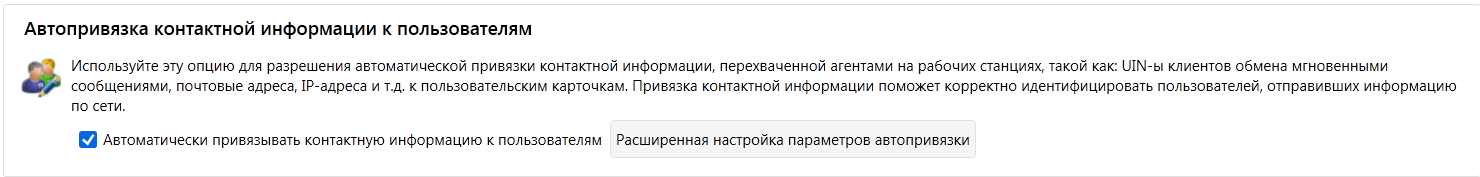
\includegraphics[scale=0.3]{pics/auto_connect.png}
        \end{center}
        \item \textbf{Как добавляется и обновляется информация о пользователях системы, если сеть организации построена на базе Active Directory/рабочей группы?}\par
        \qquad База пользователей формируется автоматически системой либо наполняется администратором при помощи Консоли администратора. Если сеть построена на базе Active Directory, то база пользователей создается и обновляется системой в автоматическом режиме. Система SecureTower позволяет произвести импорт всех пользователей из Active Directory, включая тех, чьи компьютеры не контролируются, для идентификации всех взаимосвязей контролируемых пользователей с другими сотрудниками организации. Если компьютеры сети организованы в рабочую группу, то база пользователей должна быть наполнена администратором системы вручную через Консоль администратора либо Консоль пользователя.

    \end{enumerate}
    \end{document}